\section{Introduction and Motivation}

MicroBooNE (Micro Booster Neutrino Experiment) is an experiment based at the Fermi National Accelerator Laboratory (Fermilab) that uses a large Liquid Argon Time Projection Chamber (LArTPC) to investigate the excess of low energy events observed by the MiniBooNE experiment \cite{Aguilar-Arevalo:2013pmq} and to study neutrino-argon cross-sections. MicroBooNE is part of the Short-Baseline Neutrino (SBN) physics program, along with two other LArTPCs: the Short Baseline Near Detector (SBND) and the Imaging Cosmic And Rare Underground Signal (ICARUS) detector. {\ub} also provides important research and development in terms of detector technology and event reconstruction techniques for future LArTPC experiments including DUNE (Deep Underground Neutrino Experiment).\\

\begin{figure}[ht!]
\centering
	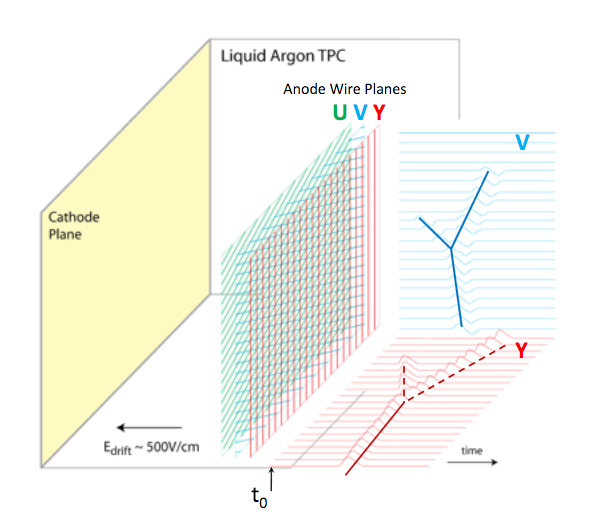
\includegraphics[width=0.4\linewidth]{Figures/detector2.png} \\
\caption{\textit{A diagram of the time projection chamber of the MicroBooNE detector \cite{lartpc}.}}\label{detector_fig}
\end{figure}

The MicroBooNE detector is currently the largest LArTPC in the United States. It consists of a rectangular time projection chamber (TPC) with dimensions 2.6 m width $\times$ 2.3 m height $\times$ 10.4 m length located 470 m away from the Booster Neutrino Beam (BNB) target. Time projection chambers, filled with a gas or liquid volume, are used to analyze particle interactions in three dimensions. The x-direction of the TPC corresponds to the drift coordinate, the y-direction is the vertical direction, and the z-direction is the direction along the beam. The amount of active liquid argon in the TPC is 89 tons, with the total cryostat containing 170 tons of liquid argon. Liquid argon is chosen to fill the volume for a variety of reasons: argon contains a high density of nucleons, which allows for a greater rate of interactions with particles within the medium; argon ionizes easily; it is transparent to itw own scintillation light; it has a high electron lifetime; and it is inexpensive.\\

Photomultiplier tubes (PMTs) and three wire planes with 3mm spacing at angles of 0, and $\pm$ 60 degrees with respect to the vertical are located in the TPC to aid with event reconstruction (Figure \ref{detector_fig}). In a neutrino interaction, a neutrino from the beam interacts with the argon and the charged outgoing child particles traverse the medium, losing energy and leaving an ionization trail. The resulting electrons drift to the anode side of the TPC, containing the wire planes, away from the negatively charged cathode plate on the opposite side. The movement of electrons induces a current in the wires, which is used to create three distinct two-dimensional views of the event. Combining these wire signals with timing information from the PMTs allows for full three-dimensional reconstruction of the event.\\


% One of the aims of MicroBooNE is to explore neutrino oscillations. For the two neutrino case, the probability that a neutrino with an initial flavor $\alpha$ will be observed as a neutrino with a different flavor $\beta$ when measured is: 

% \begin{equation}
%     P_{\alpha \rightarrow \beta}=\text{sin}^2(2\theta)\text{sin}^2(\frac{\Delta m^2 L}{4E})
% \end{equation}

% \noindent where $\theta$ is the mixing angle, $L$ is the distance from the neutrino source to the detector, $E$ is the energy of the neutrino, and $\Delta m^2$ is the neutrino squared mass difference. $\theta$ and $\Delta m^2$ are the two free parameters of interest in the above equation. The probability $P$ can be determined through a measurement of observed neutrino events compared to expected events, the distance $L$ is readily determined and constant, and $E$ can be computed from the energies of the neutrino's interaction products. 

The BNB is predominantly composed of muon neutrinos, which can undergo charge-current interactions in the TPC and produce muons. For muon tracks that are completely contained in the TPC, it is straightforward to calculate the momentum with a measurement of the length of the particle's track. Around half of muons from BNB neutrino events in {\ub} are not fully contained in the TPC, and therefore using length-based calculations for these uncontained tracks is not a possibility. The only way to compute the energy of an outgoing three-dimensional track is by means of multiple coulomb sccattering (MCS). \\

The phenomenon of multiple coulomb scattering (MCS) occurs when a charged particle enters a medium and undergoes electromagnetic scattering with the atomic nuclei. This scattering deviates the original trajectory of the particle within the material (Figure \ref{mcs_nocap_fig}). For a given energy, the scatters of a track-like particle (in terms of angular deflection relative to the track direction) form a gaussian distribution centered at zero with a standard deviation given by the Highland formula \cite{highland}: 

\begin{equation}
	\sigma_o=\frac{13.6\  \text{MeV}}{p\beta c}z\sqrt{\frac{\ell}{X_0}}\Big[1+0.0038\text{ln}\Big(\frac{\ell}{X_0}\Big)\Big]
\end{equation}\label{highland_eqtn}

\noindent where $\beta$ is the ratio of the particle's velocity to the speed of light, $\ell$ is the distance traveled inside the material, and $X_0$ is the radiation length of the target material (taken to be a constant 14 cm in liquid argon). With the Highland formula, the momentum of a track-like particle can be determined using only the 3D reconstructed track it produces in the detector, without any calorimetric information. The method by which this is done is described in detail in Section \ref{MCS_technique_section}.

\begin{figure}[ht!]
\centering
	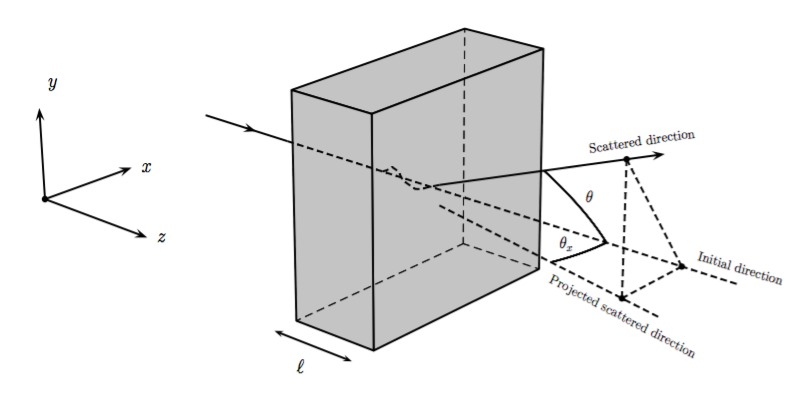
\includegraphics[width=0.5\linewidth]{Figures/mcs_nocap.png} \\
\caption{\textit{The particle's trajectory is deflected as it traverses through the material \cite{leonidas1}.}}\label{mcs_nocap_fig}
\end{figure}